\documentclass[11pt, xcolor={dvipsnames}, hyperref={colorlinks, allcolors=Blue}]{beamer}


% Packages
\usepackage{graphicx}
\usepackage{caption, subcaption}
\usepackage{tikz}
\usepackage{amsmath, amsfonts, amssymb}
\usepackage{bm}
\usepackage{booktabs}
\usepackage{apacite}
\usepackage{multirow}
\usepackage{multicol}
\usepackage{doi}
\usepackage{textpos}
\usepackage{lipsum}
\usepackage{amsfonts, amsmath}
\usepackage{wrapfig}
\usepackage{animate}
\usepackage{cleveref}


\renewcommand\doiprefix{}


\usepackage{tikz}
\usetikzlibrary{shapes, fit}





%%%%%%%%%%%%%%%%%%%%%%%%%%%%%%%%%%%%%%%%%%%%%%
% Custom commands
\newcommand\bc[1]{{\usebeamercolor[fg]{frametitle} {\textbf{#1}}}} % bold and color
\newcommand{\into}{\rightarrow}



%%%%%%%%%%%%%%%%%%%%%%%%%%%%%%%%%%%%%%%%%%%%%%
% Set Theme
\usetheme{Boadilla}
\usecolortheme{rose}

%%%%%%%%%%%%%%%%%%%%%%%%%%%%%%%%%%%%%%%%%%%%%%
% Make citation font tiny
\renewcommand{\bibliographytypesize}{\tiny}

%%%%%%%%%%%%%%%%%%%%%%%%%%%%%%%%%%%%%%%%%%%%%%
% Fonts
\usefonttheme{serif} % Serif font
\setbeamertemplate{enumerate items}[default] % Don't use bullets in enumerate.

%%%%%%%%%%%%%%%%%%%%%%%%%%%%%%%%%%%%%%%%%%%%%%%
% Remove navigation bar
\setbeamertemplate{navigation symbols}{}
%%%%%%%%%%%%%%%%%%%%%%%%%%%%%%%%%%%%%%%%%%%%%%


% Frontmatter
\title[ECON 8000 -  Lecture 6]{Lecture 6: Statistics}
\author[University of Queensland]{Robert Garrard}
\date[\today]{} 


%%%%%%%%%%%%%%%%%%%%%%%%%%%%%%%

% Common commands

% Sets
\newcommand{\R}{\mathbb{R}}
\newcommand{\N}{\mathbb{N}}
\newcommand{\Z}{\mathbb{Z}}
\newcommand{\Q}{\mathbb{Q}}
\renewcommand{\P}{\mathbb{P}}
\newcommand{\E}{\mathbb{E}}

% Symbols
\renewcommand{\epsilon}{\varepsilon}
\renewcommand{\implies}{\Rightarrow}
\newcommand{\halmos}{\hfill$\blacksquare$}

% Vector notation
\renewcommand{\a}{\mathbf{a}}
\renewcommand{\b}{\mathbf{b}}
\newcommand{\x}{\mathbf{x}}
\newcommand{\X}{\mathbf{X}}
\newcommand{\y}{\mathbf{y}}
\newcommand{\z}{\mathbf{z}}
\renewcommand{\v}{\mathbf{v}}
\newcommand{\bepsilon}{\mathbf{\varepsilon}}
\newcommand{\bbeta}{\mathbf{\beta}}

% Matrices
\newcommand{\eyetwo}{\begin{pmatrix} 1 & 0\\ 0 & 1 \\ \end{pmatrix}} % I_2 identity matrix
\newcommand{\eyethree}{\begin{pmatrix} 1 & 0 & 0\\ 0 & 1 & 0\\ 0 & 0 & 1 \end{pmatrix}} % I_3 identity matrix
\newcommand{\zerotwo}{\begin{pmatrix} 0 & 0\\ 0 & 0 \\ \end{pmatrix}} % 2x2 Zero matrix
\newcommand{\zerothree}{\begin{pmatrix} 0 & 0 & 0\\ 0 & 0 & 0\\ 0 & 0 & 0 \end{pmatrix}} % 3x3 Zero matrix


% Misc

\newcommand{\innerprod}[2]{\langle #1, #2 \rangle}


%%%%%%%%%%%%%%%%%%%%%%%%%%%%%%%%

% Tikz
\usetikzlibrary{arrows,shapes,trees, positioning}

%%%%%%%%%%%%%%%%%%%%%%%%%%%%%%

\newcounter{Lecture}
\addtocounter{Lecture}{6}

\newcounter{exercise}
\newenvironment{exercise}[1][]{\refstepcounter{exercise}\par\medskip
   \noindent {\bc{Exercise}~\bc{\theLecture.\theexercise} #1}}{\medskip}


\begin{document}

\begin{frame}
\titlepage

%\begin{picture}(0,0)
%\put(35,-50){\hbox{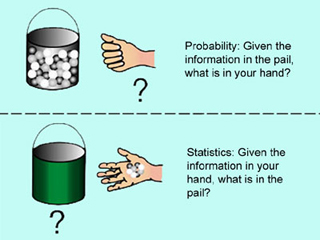
\includegraphics[width=0.8\textwidth, trim={0cm, 1cm, 0cm, 1cm}, clip]{prob_stats}}}
%\end{picture}

\end{frame}

%%%%%%%%%%%%%%%%%%%%%%%%%%%%%
\begin{frame}{Estimation}
Statistical questions typically begin in the same place:

\[\text{Let } X_1, X_2, \dots, X_n \overset{\text{iid}}{\sim} F\]

 be an independent and identically distributed (iid) sample from a distribution $F$.\bigskip

$F$ is called the \bc{data generating process}. \bigskip

We usually want to estimate a property of $F$ based on the sample.\bigskip

Often we may assume $F$ belongs to a particular family, such as $F = N(\theta, \sigma^{2})$, for which we need to estimate a parameter. This is called \bc{parametric} statistics.
\bigskip

Other times we may make no assumptions about the distribution $F$, this is called \bc{non-parametric} statistics.
\end{frame}

%%%%%%%%%%%%%%%%%%%%%%%%%%%%%
\begin{frame}{Estimation}

Let $F$ be a distribution with parameter $\theta$. An \bc{estimator} is a function of a sample from $F$.

\[\hat{\theta} = T(X_1, \dots, X_n; F)\]
\smallskip

Since it is a function of a random sample, the estimator is itself a random variable.\bigskip

Ideally, we want to use estimators whose distributions have nice properties.
\end{frame}

%%%%%%%%%%%%%%%%%%%%%%%%%%%%%
\begin{frame}{Estimation}
An estimator is \bc{unbiased} if $\E [ \hat{\theta} ]  = \theta$.\bigskip

Let $X_1, \dots, X_n \sim F$ be an iid sample from a distribution with unknown mean $\E[X] = \mu$. \bigskip

Let the \bc{sample mean} be the estimator: 
\[\bar{X} = \frac{1}{n}\sum_{i=1}^{n} X_i\]

\begin{exercise}
Show that $\hat{\theta} = \bar{X}$ is unbiased for $\mu$. Is $\hat{\theta} = X_{1}$ unbiased?
\end{exercise}
\end{frame}

%%%%%%%%%%%%%%%%%%%%%%%%%%%%%
\begin{frame}{Estimation}
Let $X_1, \dots, X_n \sim F$ be an iid sample from a distribution with unknown variance $\E[(X-\mu)^{2}] = \sigma^{2}$. \bigskip

Let the sample variance be the estimator
\[s^{2} = \frac{1}{n-1} \sum_{i} (X_{i} - \bar{X})^{2}\]
\bigskip

\begin{exercise}
\begin{enumerate}
	\item Is the sample variance unbiased for $\sigma^{2}$?
	\item What about $\frac{1}{n} \sum_{i} (X_{i} - \bar{X})^{2}$?
	\item Is $s$ unbiased for $\sigma$?
\end{enumerate}
\end{exercise}
\end{frame}
%%%%%%%%%%%%%%%%%%%%%%%%%%%%%

%%%%%%%%%%%%%%%%%%%%%%%%%%%%%
\begin{frame}{Convergence of Random Variables}

Consider a sequence of tosses of a fair coin with the random variable
\[X_{i} = \begin{cases}1 & \text{if heads}\\ 0 & \text{if tails}\end{cases}\]

After each toss, compute the mean $\bar{X}_{n} = n^{-1}\sum_{i=1}^{n} X_{i}$. This generates a sequence
\[ \{\bar{X}_{1}, \bar{X}_{2}, \bar{X}_{3}, \dots\} \]

\vfill \vfill
\bc{Question: }Does this sequence converge? (in the $\epsilon$-ball sense)

\end{frame}

%%%%%%%%%%%%%%%%%%%%%%%%%%%%%
\begin{frame}{Convergence of Random Variables}
We say that a sequence of random variables $\{X_{n}\}$ \bc{converges in probability} to $X$, written $X_{n} \overset{p}{\to} X$,  if $\forall \epsilon > 0$
\[\lim_{n\to\infty} \P(  |X_{n} - X| > \epsilon) = 0\]
\medskip

We say that a sequence of random variables $\{X_{n}\}$ \bc{converges almost surely} to $X$, written $X_{n} \overset{a.s.}{\to} X$,  if 
\[ \P( \lim_{n\to\infty} X_{n} = X) = 1\]
\medskip

We say that a sequence of random variables $\{X_{n}\}$ \bc{converges in distribution} to $X$, written $X_{n} \overset{d}{\to} X$,  if 
\[ F_{n}(x) \to F(x) \quad \forall x\]
\medskip

Convergence almost surely $\implies$ convergence in probability $\implies$ convergence in distribution

\end{frame}
%%%%%%%%%%%%%%%%%%%%%%%%%%%%%
\begin{frame}{Convergence of Random Variables}
\begin{exercise}
Show that the mean in the coin tossing example above converges in probability to $1/2$.
\end{exercise}
\vfill\vfill
\bigskip
\vfill\bigskip\vfill

\end{frame}
%%%%%%%%%%%%%%%%%%%%%%%%%%%%%

%%%%%%%%%%%%%%%%%%%%%%%%%%%%%
\begin{frame}{Convergence of Random Variables}

When trying to prove certain convergence properties, two theorems will be particularly useful:\bigskip

\begin{theorem}[Continuous Mapping Theorem]
Let $g(\cdot)$ be a continuous function. Then 
\begin{align*}
& X_{n} \overset{d}{\to} X \implies g(X_{n}) \overset{d}{\to} g(X)\\	
& X_{n} \overset{p}{\to} X \implies g(X_{n}) \overset{p}{\to} g(X)\\	
& X_{n} \overset{a.s.}{\to} X \implies g(X_{n}) \overset{a.s.}{\to} g(X)\\	
\end{align*}
\end{theorem}

Consequently, the usual arithmetic operations preserve convergence. And 
\[\mathbf{A}_{n} \to \mathbf{A} \implies \mathbf{A}_{n}^{-1} \to \mathbf{A}^{-1}\]
\end{frame}
%%%%%%%%%%%%%%%%%%%%%%%%%%%%%
\begin{frame}{Convergence of Random Variables}

\begin{theorem}[Slutsky's Theorem]
Let $X_{n} \overset{d}{\to} X$ and $Y_{n} \to c$.
\begin{align*}
&X_{n} + Y_{n} \overset{d}{\to} X + c\\
& X_{n}Y_{n} \overset{d}{\to} Xc\\
& X_{n}/Y_{n} \overset{d}{\to} X / c, \text{provided $c \not 0$ }.
\end{align*}
\end{theorem}

In addition, if $\mathbf{x}_{n} \overset{d}{\to} \mathbf{x}$ and $\mathbf{A}_{n} \overset{p}{\to} \mathbf{A}$, then $\mathbf{A}_{n}\mathbf{x}_{n} \overset{d}{\to} \mathbf{A}\mathbf{x}$.
\end{frame}

%%%%%%%%%%%%%%%%%%%%%%%%%%%%%
\begin{frame}{Consistency}

An estimator, $\hat{\theta}$, is \bc{consistent} for a parameter $\theta$ if $\hat{\theta} \overset{p}{\to} \theta$.

\begin{exercise}
Let $X_{1}, \dots, X_{n} \sim F$ be an iid sample drawn from a distribution with finite mean $\mu = \E[X]$ and variance $\sigma^{2}$. Show that the sample mean, $\bar{X}$ is a consistent estimator of the population mean, $\mu$.
\end{exercise}
\vfill\vfill
\bigskip\vfill\bigskip\vfill
\end{frame}
%%%%%%%%%%%%%%%%%%%%%%%%%%%%%
\begin{frame}{Laws of Large Numbers}

\begin{theorem}[Khinchin's weak law of large numbers]
Let $X_{1}, \dots, X_{n} \sim F$ be an iid sample from a distribution with mean $\mu$. 
\[\bar{X}_{n} = \frac{1}{n}\sum X_{i} \overset{p}{\to} \mu\]
\end{theorem}
\bigskip

\begin{theorem}[Kolmogorov's strong law of large numbers]
Let $X_{1}, \dots, X_{n} \sim F$ be an iid sample from a distribution with finite mean $\mu$ and variance $\sigma^{2}$. 
\[\bar{X}_{n} \overset{a.s.}{\to} \mu\]
\end{theorem}

\end{frame}

%%%%%%%%%%%%%%%%%%%%%%%%%%%%%
\begin{frame}{Laws of Large Numbers}
\begin{exercise}
Let $X_{1}, \dots, X_{n} \sim F$, $\mathrm{Var}(X) = \sigma^{2} < \infty$. Show that $s = \sqrt{\frac{1}{n-1} \sum (X_{i} - \bar{X})^{2}} \overset{p}{\to} \sigma$.
\end{exercise}

\vfill\vfill
\end{frame}

%%%%%%%%%%%%%%%%%%%%%%%%%%%%%
\begin{frame}{Sampling Distribution}

Recall that a statistic is itself a random variable and has a corresponding probability distribution.\medskip

However, the statistic may have a different distribution depending on the sample size.\medskip

Let $\X = (X_1, \dots, X_n)$ be a random sample from distribution $F$. Let $\hat{\theta} = \hat{\theta}(\X)$ be a statistic. The \bc{sampling distribution} of $\hat{\theta}$ is
\[ F_{\theta_{n}}(\tau) = \P_{n} ( \hat{\theta}(\X) \leq \tau) \]


\end{frame}

%%%%%%%%%%%%%%%%%%%%%%%%%%%%%
\begin{frame}{Sampling Distribution}

\begin{block}{Proposition}
Let $X_1, \dots, X_n \sim N(\mu, \sigma^{2})$. The sample mean, $\bar{X}$, has the following sampling distribution.

\[ \sqrt{n}(\bar{X} - \mu) \sim N(0, \sigma^{2})\]

or equivalently
\[\sqrt{n} \frac{\bar{X} - \mu}{\sigma} \sim N(0,1)\]
\end{block}
Proof is a tutorial exercise.
\end{frame}

%%%%%%%%%%%%%%%%%%%%%%%%%%%%%
\begin{frame}{Central Limit Theorems}

Usually we won't be able to characterize the finite sample distribution of a statistic exactly. \medskip

Instead, we may be able to approximate it with an \bc{asymptotic} distribution.

\begin{theorem}[Lindeberg-L\'{e}vy CLT]
Let $X_{1}, \dots X_{n} \overset{iid}{\sim} F$, with $\E[X] = \mu$ and $\mathrm{Var}(X) = \sigma^{2}$, both finite. Let $\bar{X}_{n} = \frac{1}{n}\sum X_{i}$. 

\[\sqrt{n} (\bar{X}_{n} - \mu) \overset{d}{\to} N(0,\sigma^{2})\]

or equivalently

\[\sqrt{n} \frac{(\bar{X}_{n} - \mu)}{\sigma} \overset{d}{\to} N(0,1)\]
\end{theorem}

\end{frame}

%%%%%%%%%%%%%%%%%%%%%%%%%%%%%
\begin{frame}{Central Limit Theorems}

\begin{theorem}[Multivariate CLT]
Suppose $\X$ is a random vector with finite mean $\mathbf{\mu}$ and variance $\mathbf{\Sigma}$. Then
\[ \sqrt{n} \left ( \bar{\X}_n - \mathbf{\mu}\right) \overset{d}{\rightarrow} N(\mathbf{0}, \mathbf{\Sigma})\]


\end{theorem}
\end{frame}

%%%%%%%%%%%%%%%%%%%%%%%%%%%%%
\begin{frame}{Central Limit Theorems}
We'll sketch out a proof of the CLT using moment generating functions.\medskip

Let $Y_{i} = \frac{X_{i} -  \mu}{\sigma}$. Then $\E[Y_{i}] = 0$, $\E[Y_{i}^{2}] = 1$.\bigskip

$\bar{X} = n^{-1/2}\sum Y_{i}$. Therefore, $M_{\bar{X}}(t) = \left [ M_{Y_{i}}(\frac{t}{\sqrt{n}}) \right]^{n}$.\bigskip

Performing a Taylor expansion about 0 gives: $M_{Y_{i}}(t) = 1 + \frac{t^{2}}{2} + \mathcal{O}\left(t^{3}\right)$ \bigskip

$M_{\bar{X}}(t) = \left [ M_{Y_{i}}(\frac{t}{\sqrt{n}}) \right]^{n} = \left[1 + \frac{t^{2}/2}{n} + \mathcal{O}\left( \frac{t^{3}}{n^{3/2}} \right) \right]^{n} \to e^{t^{2}/2}$

\end{frame}

%%%%%%%%%%%%%%%%%%%%%%%%%%%%%
\begin{frame}{Inference - Hypothesis Tests}
We care about some unknown parameter $\theta$.\bigskip

 Suppose we have a consistent estimator, $\hat{\theta}_{n} \overset{p}{\to} \theta$.\bigskip

Suppose we know the distribution of this estimator $\P(\hat{\theta}_{n} \leq x)$.\bigskip

Can we make some claims about $\theta$ with confidence?\bigskip

E.g., ``the average height of an Australian adult is above 1m'', or ``smoking a pack of cigarettes a day increases your risk of lung cancer''.

\end{frame}

%%%%%%%%%%%%%%%%%%%%%%%%%%%%%
\begin{frame}{Inference - Hypothesis Tests}

Hypothesis testing is always about trying to reject some sort of hypothesis as false. If you were to hypothesise what you were trying to prove, then the hypothesis might be retained for one of two reasons:\bigskip

\begin{enumerate}[1.]
\item The hypothesis is true.
\item You don't have a sufficient sample size to resolve the difference between your hypothesis and the true value. It may be the case that you would retain pretty much any hypothesis you started with!
\end{enumerate}
\bigskip

Typically our hypothesis will be one of $\theta = 0$, $\theta \leq 0$, or $\theta \geq 0$.


\end{frame}
%%%%%%%%%%%%%%%%%%%%%%%%%%%%%

\begin{frame}{Inference - Hypothesis Tests}

So we construct a \bc{null hypothesis} which we wish to disprove.\bigskip

 This is usually a statement about one or more parameters of a distribtuion and is typically written 

\[H_{0}: \theta = \theta_0\]
\bigskip

In the event that we reject the null hypothesis, we retain an \bc{alternative hypothesis}, which is usually the converse of the null.

\[H_{1}: \theta \not= \theta_0\]
\end{frame}

%%%%%%%%%%%%%%%%%%%%%%%%%%%%%

\begin{frame}{Inference - Hypothesis Tests}

Once we know what we're trying to reject, we need to set a tolerance for which we're willing to make mistakes.\bigskip

We pick an $\alpha$, the \bc{(nominal) level} of the test. Often $\alpha = 0.05$.\bigskip

We then need to pick a \bc{test statistic}, which is usually a function of an estimator (which is itself a function of the sample).  E.g.

\[T = T(\mathbf{X}) = \sqrt{n}\frac{(\hat{\theta} - \theta_{0})}{\hat{\sigma}} \]


\end{frame}
%%%%%%%%%%%%%%%%%%%%%%%%%%%%%

\begin{frame}{Inference - Hypothesis Tests}

A typical hypothesis test proceeds as follows.

\begin{enumerate}[1.]
\item Have a parameter of interest and an estimator for it.
\item State the null and alternative hypotheses in terms of your parameter of interest. 
\item Choose a test statistic.
\item If the null were \emph{true}, what would the sampling distribution of the test statistic be?
\item Find the appropriate quantiles of the sampling distribution. These are your \bc{critical values}.
\item Calculate the value of your test statistic from your sample. Compare to the critical value.
\item If the value of the statistic is greater than the critical value, reject the null and retain the alternative. Else retain the null.
\end{enumerate}
\end{frame}
%%%%%%%%%%%%%%%%%%%%%%%%%%%%%
\begin{frame}{Inference - Hypothesis Tests}
\begin{block}{Example}
Let $X_1, \dots, X_{10} \sim N(\mu, 4)$. We wish to test
\[H_{0}: \mu = 1 \ \text{vs} \ H_{A}: \mu \not = 1\]
at the 5\% level. We find a sample mean of $\bar{X} = 2.3$. Under the null hypothesis, we have the following sampling distribution.
\[ \sqrt{10}\frac{\bar{X} - 1}{2} \sim N(0,1)\]
We have a two sided test, so the $\alpha/2$ and $1-\alpha/2$ quantiles are $-1.96$ and $1.96$ respectively. Let's calculate our test statistic given our observed sample mean.
\[ \sqrt{10}\frac{2.3 - 1}{2} = 2.05\]
$2.05 > 1.96$, so we may reject the null and retain the alternative.
\end{block}
\end{frame}
%%%%%%%%%%%%%%%%%%%%%%%%%%%%%
%%%%%%%%%%%%%%%%%%%%%%%%%%%%%
\begin{frame}{Inference - Hypothesis Tests}

A test might incorrectly reject a null hypothesis that is in fact true. This is called a \bc{type-I error} (or \bc{false discovery}). \bigskip

The probability of a type-I error, $\alpha$, is called the \bc{size} of the test.\bigskip

A test m ight incorrectly retain a null hypothesis that is in fact false. This is called a \bc{type-II error}.\bigskip

The probability of a type-II error, $\beta$, is called the \bc{power} of the test.\bigskip

\end{frame}

%%%%%%%%%%%%%%%%%%%%%%%%%%%%%
\begin{frame}{Inference - Hypothesis Tests}
If we have correctly specified the distribution of the test statistic, and used the correct critical values, then the size of the test will be equal to the nominal level.\bigskip

Note that the distribution will not always be correctly specified, since we may be using asymptotic approximations.\bigskip

If the size of a test is less its nominal level, it is called \bc{conservative}.\bigskip

If the size of a test is greater than its nominal level, it is called \bc{anti-conservative}.
\end{frame}

%%%%%%%%%%%%%%%%%%%%%%%%%%%%%
\begin{frame}{Inference - Hypothesis Tests}

Finding a test statistic with a known distribution can be challanging. \bigskip

In particular, to extract critical values, we'd prefer that the distribution not depend on any unknown parameters (\bc{nuisance parameters}). \bigskip

Such distributions are called \bc{pivotal}. \bigskip

\begin{exercise}
\begin{enumerate}
	\item Let $X_1, \dots, X_n \sim N(\mu_X, \sigma^2)$ and $Y_1,\dots, Y_n\sim N(\mu_Y, \sigma^2)$ be samples drawn from two distributions with a known common variance. We wish to test the hypothesis $H_{0}: \mu_{X} \leq \mu_{Y}$ against the alternative $H_{1}: \mu_{X} > \mu_{Y}$. What might make a good test statistic?	
\end{enumerate}
\end{exercise}

\end{frame}

%%%%%%%%%%%%%%%%%%%%%%%%%%%%%
\begin{frame}{Inference - Hypothesis Tests}

Recall our unbiased estimator of the population variance

\[s^2 = \frac{1}{n-1} \sum_{i=1}^{n} \left ( X_{i} - \bar{X} \right )^2\]

We'll need the following fact.

\begin{block}{Proposition}
Let $X_1, \dots, X_n \overset{iid}{\sim} N(\mu, \sigma^2)$.
\[ \frac{(n-1)s^2}{\sigma^2} \sim \chi^2(n-1)\] 
\end{block}

\end{frame}
%%%%%%%%%%%%%%%%%%%%%%%%%%%%%
%%%%%%%%%%%%%%%%%%%%%%%%%%%%%
\begin{frame}{Pivotal Quantities}
Let $X_{1}, \dots, X_{n} \sim N(\mu, \sigma^{2})$, where both $\mu$ and $\sigma^{2}$ are unknown. \bigskip

If we appeal to the central limit theorem, we get

\[\sqrt{n}(\bar{X} - \mu) \sim N(0, \sigma^{2})\]

But we don't know $\sigma^{2}$!\bigskip

We can make this statistic pivotal by \bc{studentizing} it. 

\end{frame}

%%%%%%%%%%%%%%%%%%%%%%%%%%%%%
\begin{frame}{Pivotal Quantities}
\begin{block}{Proposition}
Let $X_1, \dots, X_n \overset{iid}{\sim} N(\mu, \sigma^2)$.
\[ \sqrt{n} \frac{\bar{X} - \mu}{s} \sim t(n-1)\]
\end{block}
\textit{Proof:}

\begin{align*}
\sqrt{n} \frac {\bar{X} - \mu}{s} =& \frac{\sqrt{n} \frac{\bar{X} - \mu}{\sigma}}{\frac{s}{\sigma}} = \frac{\sqrt{n} \frac{\bar{X} - \mu}{\sigma}}{\sqrt{\frac{s^2}{\sigma^2}}}
= \frac{\sqrt{n} \frac{\bar{X} - \mu}{\sigma}}{\frac{(n-1)s^2}{\sigma^2}/(n-1)}
\end{align*}
Recall the numerator is $N(0,1)$. The denomitator is $\chi^2(n-1)/ (n-1)$. And by definition
\[\frac{N(0,1)}{\sqrt{\chi^2(n-1)/(n-1)}} \sim t(n-1)\]


\end{frame}

%%%%%%%%%%%%%%%%%%%%%%%%%%%%%
\begin{frame}{Pivotal Quantities}
Quantities that converge to a pivotal distribution are called \bc{asymptotically pivotal}.

\begin{block}{Proposition}
Let $X_1, \dots, X_n \overset{iid}{\sim} F$, $\mathrm{Var}(X) = \sigma^{2} < \infty$.
\[ \sqrt{n} \frac{\bar{X} - \mu}{s} \overset{d}{\to} N(0, 1)\]
\end{block}
\textit{Proof:}\\
$X_{n} = \sqrt{n}(\bar{X} - \mu)$, $Y_{n} = s_{n}$.\medskip

$X_{n} \overset{d}{\to} N(0, \sigma^{2})$. $Y_{n} \overset{p}{\to} \sigma$.\medskip

$X_{n} / Y_{n} \overset{d}{\to} \frac{1}{\sigma}N(0, \sigma^{2}) = N(0, 1)$.
\end{frame}

%%%%%%%%%%%%%%%%%%%%%%%%%%%%%
\begin{frame}{Confidence Intervals}

A $1- \alpha$ \bc{confidence interval} for a parameter $\theta$ is an interval $C_{n} = (a, b)$  such that

\[\P_{\theta}(\theta \in C_{n}) \geq 1 - \alpha\]

That is, it's an interval that traps $\theta$ with probability $1-\alpha$. We call $1-\alpha$ the \bc{coverage} of the interval.\bigskip

\underline{$\theta$ is fixed, it's $C_{n}$ that's random!}

\end{frame}
%%%%%%%%%%%%%%%%%%%%%%%%%%%%%
\begin{frame}{Confidence Intervals}

For estimators that are asymptotically normal, such that $\sqrt{n}\frac{(\hat{\theta} - \theta)}{\hat{\sigma}} \overset{d}{\to} N(0, 1)$, we'll typically construct the interval as

\[C_{n} = \left( \hat{\theta} - z_{1-\alpha/2}\frac{\hat{\sigma}}{\sqrt{n}},\ \hat{\theta} + z_{\alpha/2}\frac{\hat{\sigma}}{\sqrt{n}}  \right)\]
\bigskip

where $z_{\alpha/2}$ is the $\alpha/2$ quantile of the normal distribution.

\vfill\vfill \bigskip
\begin{exercise}
Show that the above interval has asymptotic coverage $1-\alpha$.
\end{exercise}

\end{frame}


%%%%%%%%%%%%%%%%%%%%%%%%%%%%%
\begin{frame}{Regression}

Regression models attempt to explain an outcome variable in terms of a set of predictors. \bigskip

We'll use be given a set of $n$ obervations on $p$ predictors:  $(y_{i}, \mathbf{x}_{i}^{\prime})_{i=1}^{n}$.\bigskip

We'll assume independence across samples, $i$, but $y_{i}$ and $\mathbf{x}_{i}^{\prime}$ are jointly distributed.\bigskip

Our objective is to find a function $f(\cdot)$ that explains the outcome in terms of the predictors: $y_{i} = f(\mathbf{x}_{i}^{\prime}) + \epsilon_{i}$.\bigskip

For a few reasons, we'll restrict $f(\cdot)$ to be a linear combination of the predictors: $y_{i} = \beta_{1}x_{1} + \dots + \beta_{p} x_{p} + \epsilon_{i}$.\bigskip

Note: you can allow a constant by setting $x_{1} = 1$.
\end{frame}
%%%%%%%%%%%%%%%%%%%%%%%%%%%%%
\begin{frame}{Regression Assumptions}

We're given a sample of $n$ iid draws from a joint distribution $(y_{i}, \mathbf{x}_{i}^{\prime}) \sim F$.\bigskip

Let's make some highly spurious assumptions, and see what traction we can get:

\begin{block}{Gauss-Markov Assumptions}
\begin{enumerate}
	\item The true DGP is linear: $y = X\beta + \epsilon$. (linearity)
	\item $X$ is full column rank. (no multicollinearity)
	\item $\E[\epsilon_{i} \ | \ X] = 0$. (strict exogeneity)
	\item $\E[\epsilon_{i}^{2} \ | X] = \sigma^{2}$. (spherical errors)

\end{enumerate}
\end{block}

\end{frame}
%%%%%%%%%%%%%%%%%%%%%%%%%%%%%
\begin{frame}{Least Squares}
Now we have a linear model $y = X\beta + \epsilon$, and a parameter $\beta$ we need to estimate. How?\bigskip

\[\hat{\beta}_{OLS} = \underset{\beta}{\text{argmin}} \ ||y - X\beta||_{2}^{2}\]
\bigskip

We've seen previously that the solution to this minimization problem is 

\[\hat{\beta}_{OLS} = (X^{\prime}X)^{-1}X^{\prime}y\]

\end{frame}

%%%%%%%%%%%%%%%%%%%%%%%%%%%%%
\begin{frame}{Least Squares}

\begin{theorem}[Gauss-Markov Theorem]
Under the Gauss-Markov assumptions, the OLS estimator is the \bc{best linear unbiased estimator}.
\end{theorem}
\bigskip

\begin{exercise}
\begin{enumerate}
	\item Show that the OLS estimator is unbiased.
	\item Show that the OLS estimator is consistent.
	\item Show that the OLS estimator is asymptotically normal.
\end{enumerate}
\end{exercise}

\end{frame}
%%%%%%%%%%%%%%%%%%%%%%%%%%%%%
%%%%%%%%%%%%%%%%%%%%%%%%%%%%%
\begin{frame}{Learning Outcomes}

That's a lot already, but there's so much more good stuff! We didn't even touch on: maximum likelihood, method of moments, delta method, shrinkage estimation, kernel density estimation, etc.
\bigskip

\bc{You should be able to:}

\begin{enumerate}
	\item Determine the bias of a given estimator.
	\item Apply the CMT and Slutsky's theorem.
	\item Determine consistency of an estimator using LLN.
	\item Apply the CLT to show asymptotic normality.
	\item Conduct a hypothesis test.
	\item Construct a confidence interval.
	\item Estimate regression coefficients with OLS.
\end{enumerate}

\end{frame}
\end{document}	